\begin{figure}[!Hhtb]
  \centering
  \subfigure[Barrel.]{\label{fig:res_qpt_vs_pt_combined_barrel}
    \ifpdf
    \epsfig{file=fig/ellipses/BarrelPtRes,clip,width=0.45\linewidth,angle=0}
    \else
    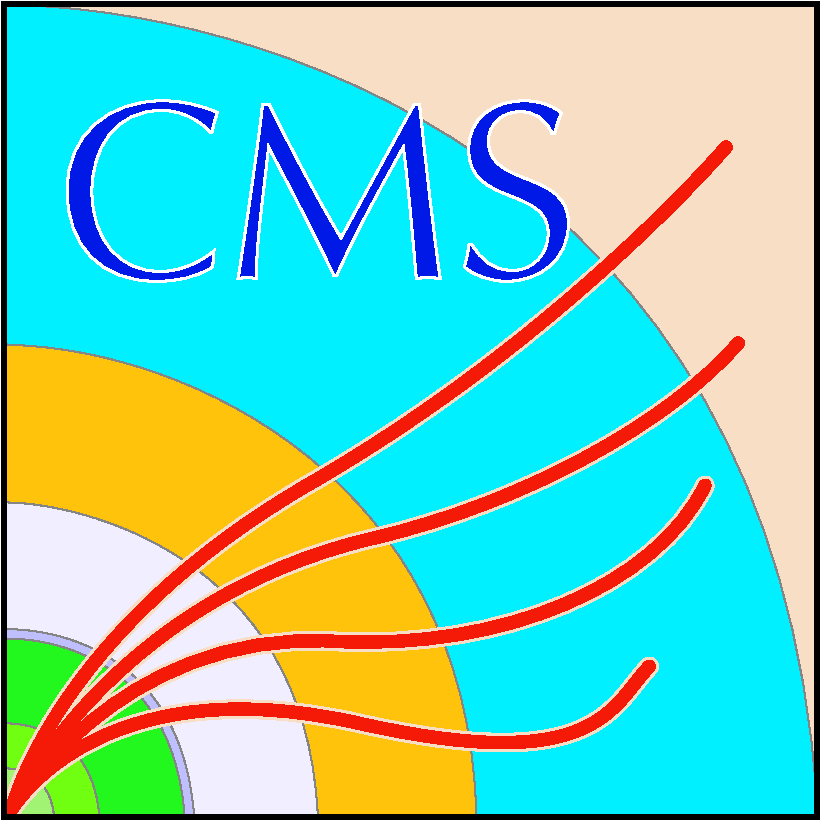
\epsfig{file=CMScol,clip,width=0.45\linewidth}
    \fi
  }
  \subfigure[Overlap.]{\label{fig:res_qpt_vs_pt_combined_overlap}
    \ifpdf
    \epsfig{file=fig/ellipses/OverlapPtRes,clip,width=0.45\linewidth,angle=0}
    \else
    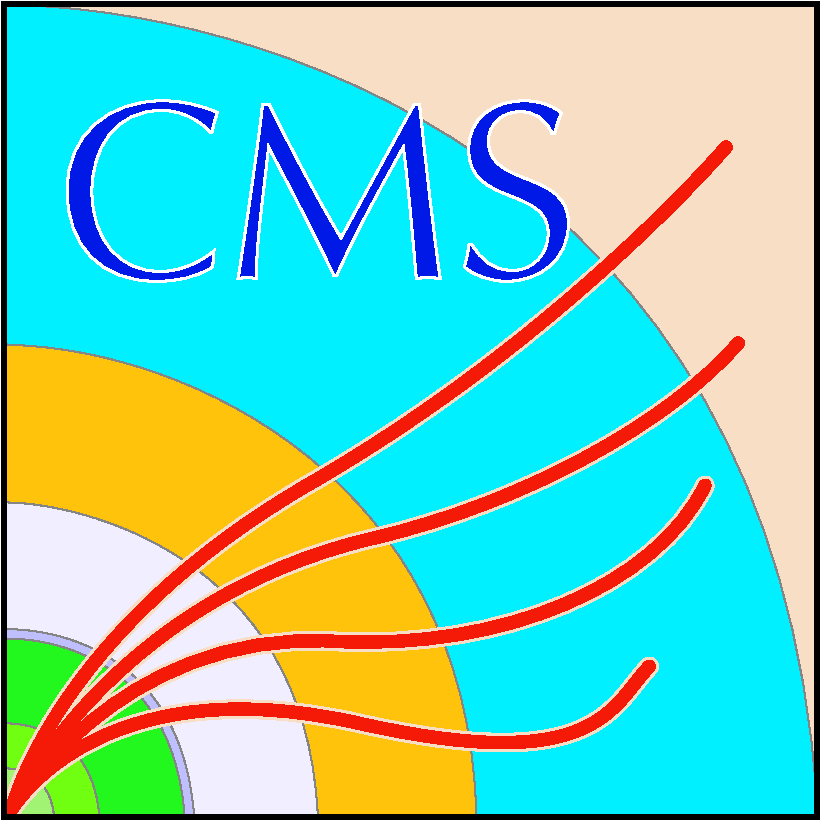
\epsfig{file=CMScol,clip,width=0.45\linewidth}
    \fi
  }
  \subfigure[End-caps.]{\label{fig:res_qpt_vs_pt_combined_endcap}
    \ifpdf
    \epsfig{file=fig/ellipses/EndcapsPtRes,clip,width=0.45\linewidth,angle=0}
    \else
    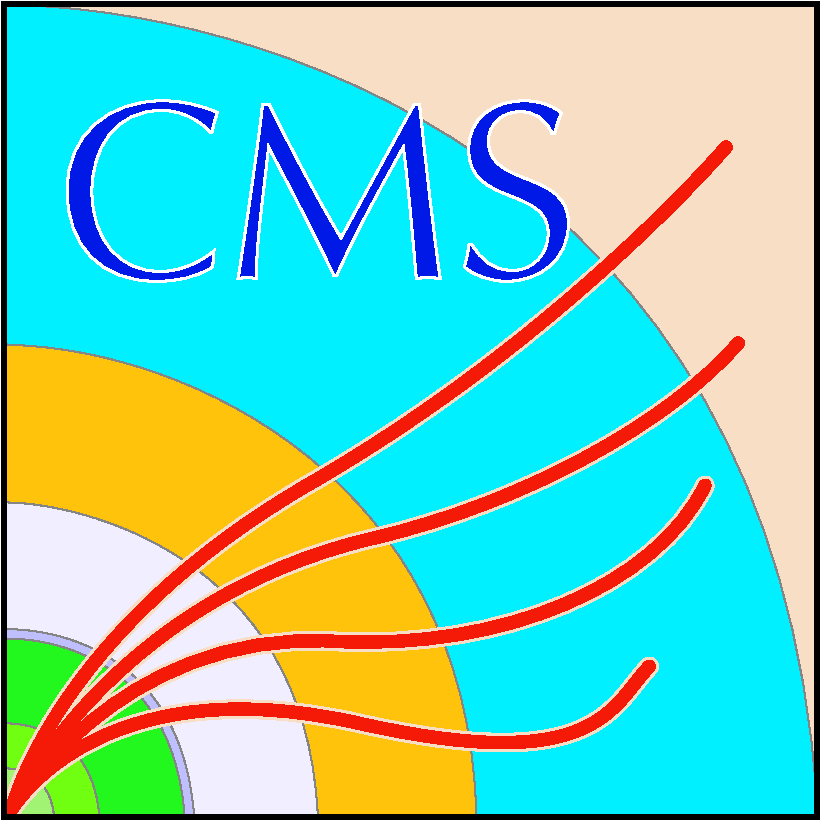
\epsfig{file=CMScol,clip,width=0.45\linewidth}
    \fi
  }
  \caption[Comparison of the $q/\pt$ resolution for the tracker system, the muon system, and the combined systems]{Resolution on $q/\pt$ with the tracker alone, with the muon
    spectrometer alone and with the full CMS tracking system, as a
    function of \pt. \label{fig:sta_tk_glb_sim_res_qpt}}  
\end{figure}
